% This version of CVPR template is provided by Ming-Ming Cheng.
% Please leave an issue if you found a bug:
% https://github.com/MCG-NKU/CVPR_Template.

%\documentclass[review]{cvpr}
\documentclass[final]{cvpr}

\usepackage{times}
\usepackage{epsfig}
\usepackage{graphicx}
\usepackage{amsmath}
\usepackage{amssymb}

\usepackage{biblatex} %Imports biblatex package
\addbibresource{references.bib}

% Include other packages here, before hyperref.

% If you comment hyperref and then uncomment it, you should delete
% egpaper.aux before re-running latex.  (Or just hit 'q' on the first latex
% run, let it finish, and you should be clear).
\usepackage[pagebackref=true,breaklinks=true,colorlinks,bookmarks=false]{hyperref}


\def\cvprPaperID{****} % *** Enter the CVPR Paper ID here
\def\confYear{MVA 2022}
%\setcounter{page}{4321} % For final version only


\begin{document}

%%%%%%%%% TITLE
\title{Multi-lingual contradiction detection \\ \small{Final project report - MVA Deep Learning course}}

\author{Jérémie Dentan\\
École Polytechnique\\
{\tt\small jeremie.dentan@polytechnique.org}
% For a paper whose authors are all at the same institution,
% omit the following lines up until the closing ``}''.
% Additional authors and addresses can be added with ``\and'',
% just like the second author.
% To save space, use either the email address or home page, not both
\and
Alicia Rakotonirainy\\
CentraleSupélec\\
{\tt\small alicia.rakotonirainy@student-cs.fr}
}

\maketitle


%%%%%%%%% ABSTRACT
\begin{abstract}
    Textual entailment recognition consists in deciding, given two excerpts of texts, whether the meaning of one of them is entailed (i.e. can be inferred) from the other. On the other hand, multi-lingual text processing consists in processing texts in different languages. This task is known to be difficult, especially because of the small amount of data available in some languages.

    In this project, we deal with both of those challenges: we perform textual entailment detection between pairs of text from a wide range of languages. More precisely, we trained algorithms to classify those pairs in three classes: entailment, contradiction, and neutral, with the objective of maximizing the weighted accuracy of this multiclass classification task.
    
    To address this challenge, we used the most recent pretrained Large Language Models (LLMs, especially BERT and XML-R) and fine-tuned them on our specific data and task. Then, to improve the LLM baseline predictions, we computed and added new relevant features and fed a XGBoost classifier with both the LLM predictions and those features to get the final prediction. 

    After applying our stacking strategy on the validation set, we achieved an increase of 3\% accuracy as compared to the LLMs predictions baseline.

\end{abstract}

Our code for the training and the evaluation is accessible  \href{https://github.com/DentanJeremie/contradictionDetection.git}{here}.

%%%%%%%%% BODY TEXT
\section{Introduction}

Our project deals both with textual entailment and multilingual text processing. We will present those notions, as well as their real-world applications.

\subsection{Textual entailment.}

Textual entailment, also known as contradiction detection or natural language inference, is a critical task in Natural Language Understanding, as it has a wide range of applications. It consists in deciding, given two excerpts of texts, whether the meaning of one of them can be inferred from the other. In the example below, sentence A entails sentence B : 

\begin{itemize}
    \item A : In Moria you will find the remains of a huge Roman aqueduct.

    \item B : There is something special to see in the village of Moria.
\end{itemize}

This task is part of the famous GLUE benchmark and leaderboard, and has received a lot of attention in recent years. Typically, textual entailment is not used for itself but as part of a larger system where it is needed. here are some example of larger systems using textual entailment:

\begin{itemize}
    \item Event prediction. When one tries to predict an event based on textual data, entailment has to be filtered. Indeed, for such a prediction to be interesting, it should not be entailed directly in the present text. For example, if we read in a newspaper that "3 children were killed in a bus accident in Paris", the prediction "There was a traffic accident in Paris" is true, but we want to filter out this prediction because it is already entailed in the first sentence. Thus, filtering textual entailment can be used as post-processing to predict something really new and interesting for humans. \cite{Radinsky2013}.
    
    \item Event argument extraction. This task consists in extracting structured information from unstructured text for a particular event of interest. To illustrate this, let's take an example from \cite{Sainz2022}. We have the sentence "In 1997, the company hired John D. Idol to take over as chief executive". Then, we use several templates specific to this situation to generate sentences for the different roles of John D. Idol, such as "John D. Idol was hired" (template "personal start position"), "John D. Idol hired someone" (template "entity start position"), etc. Then, looking for the generated sentence that is best entailed by the original one, we know which template applies the best and thus we can know the role of John D. Idol in the original sentence.
\end{itemize}

\subsection{Multi-lingual text processing.}

Similarly to textual entailment, multi-lingual text processing is a core task of Natural Language Understanding (NLU), which includes a wide range of applications and has recieved a lot of attention during the past years.

One of the biggest difficulty with multi-lingual text processing it the low availability of data, and especially labelled data, in low-resource languages. For example, over the 7000+ languages spoken worldwide, only 30 of them represent individually more than 99.9\% of the texts online \cite{webLanguages}. Figure \ref{fig:percentageLanguages} represents the percentage of use of the languages on the internet, with the data of \cite{webLanguages}. We clearly see that some common languages have huge resources available online to train large language models, whereas other languages are nearly absent.

\begin{figure}[ht]
	\centering
	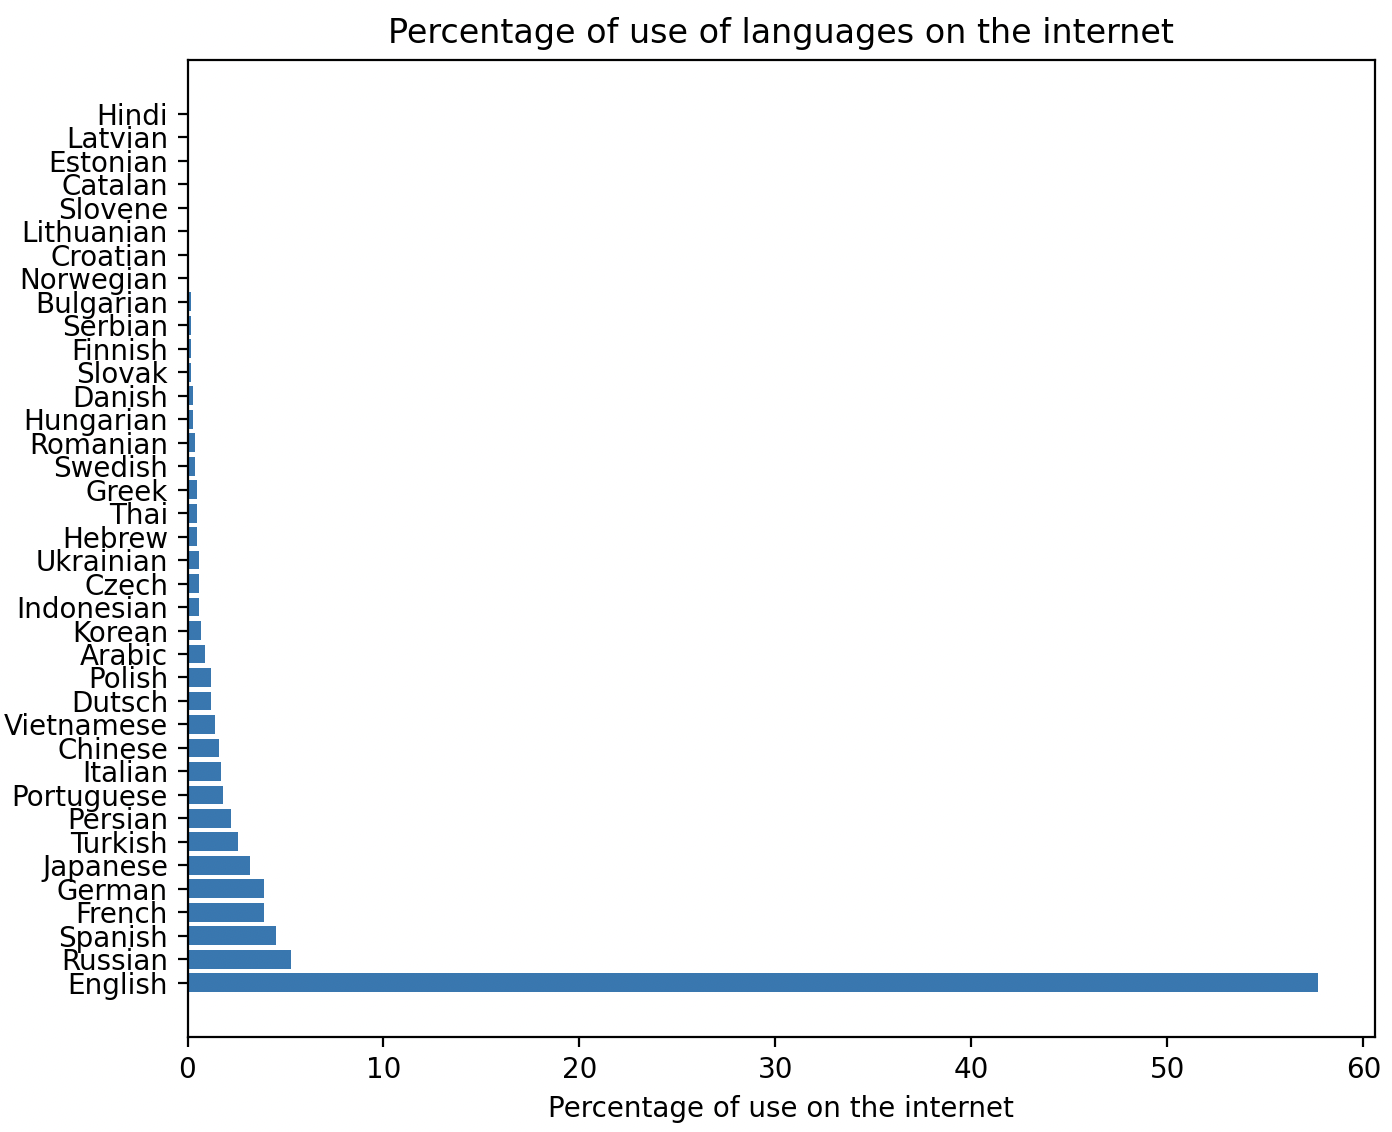
\includegraphics[width=\columnwidth]{figures/percentageLanguages.png}
	\caption{Percentage of use of languages on the internet. All other languages represent less that 0.1\% of the texts online}
    \label{fig:percentageLanguages}
\end{figure}

Mutli-lingual text processing has countless applications. For example, it can be used to leverage a model trained on a specific NLP task in english with resources in other languages. For example, in the case of Named Entity Recognition (NER) with biomedical textual data in Spanish, instead of specifically train a network for this task in Spanish, which requires a lot a data and computation resources, the authors of \cite{Kai2019} have combined a network trained for NER on English biomedical literature, and a multilingual BERT model pretrained on general domain texts. 

\section{Formal description of the problem}

We focus on the problem of \textit{textual entailment recognition}. The main input to a textual entailment recognizer is a pair of sentences ; the first one is the \textit{premise}, the second one the \textit{hypothesis}. The output is a label indicating whether the premise entails the meaning of the hypothesis, or if the two sentences are unrelated, or contradict each other. We want to maximize the weighted accuracy of this multiclass classification task.


\section{Related work}

\subsection{Logic-based Approaches}

A first possibility is to convert sentences into logical formulae, and check for logical entailment (denoted as $\models$) \cite{Rocha2018}. If logical meaning representations of the premise and hypothesis are $\phi_P$ and $\phi_H$, then the pair $(P,H)$ is a correct textual entailment pair if and only if ($\phi_T \wedge B) \models \phi_H$ where $B$ is a knowledge base assumed to be shared by all language users. In practice, this solution commonly involves the use of theorems provers (see \cite{Tatu2006} for an example). One of the main difficulty relies in the choice of a reasonably complete $B$. These formal logic approaches were extensively used before the release of bigger size datasets that encouraged more learning-centered approaches, which in turn outperformed the so far existing state-of-the-art \cite{jiang2015}.

\subsection{Vector Space models and Deep Learning Approaches}

State-of-the-art systems for textual entailment detection typically follow a standard NLP pipeline. In those methods, each word is mapped to a vector, such that "similar" words have a similar encoding. Textual entailment can then be detected by measuring the distance of the vectors of the premise and hypothesis, for example by computing their cosine similarity. For instance, \cite{bowman2015} used a feed-forward deep neural network to compute an embedding vector for the premise and the hypothesis. The two vectors are then fed into a multi-layer neural network, that is trained to perform the classification. 

\cite{jiang2015} proposed a modification to this latter method. They leveraged the issue of having a single embedding vector for both the premise and the hypothesis, thus attributing the same level of importance to all words in the sentence (they assume that stop words are presumably less important than content words for instance). In their model, their prediction is not based on whole sentence embedding of the premise and the hypothesis ; instead, they perform word-by-word matching of the hypothesis with an attention-weighted representation of the premise. Intuitively, if we see for instance that the subject of the hypothesis does not match the subject of the premise, we have a high probability to have a contradiction or a neutral relationship.

A few works have exploited the addition of specialised features, such that negation detection \cite{androu2009}, logical inference techniques \cite{bos2005} or semantic similarity \cite{lai2014}. Authors also used lexical features (e.g. words overlap or substring matching), as well as syntactic features (e.g. adverbs, punctuation marks...) or semantic features (e.g. similarity metrics) \cite{Rocha2018}.

For the english language, several challenges have been published : eight RTE Challenges $\cite{dagan2005}$ between 2005 and 2013, SemEval Task 1 \cite{marelli2014} or RepEval 2017 \cite{nangia2017}. To the best of our knowledge, no vast multilingual challenge have yet been released, and the vast majority of recently published papers on textual entailment detection were evaluated on english corpora.

In this project we therefore chose the approach exploiting additionnal specialised features, by creating new semantic features and adapting a stacking method. Given the lack of study of textual entailment on multilingual datasets, we decided to evaluate our algorithm on a multilingual dataset containing fifteen languages.

\textbf{The principal goal of this work was to evaluate if the addition of our new specialised features increases the performances of a simple BERT classification, in the case of a multilingual dataset.}

\section{Our method}

\subsection{Our datasets}

We took our datasets from a Kaggle competition \cite{competition}. The datasets provided consists in a train set (12.120 pairs of sentences) and a validation set (5.195 pairs of sentences), as well as a submission sample for the competition (for which true labels are not given, but we can evaluate our model directly online). 

Figure \ref{header} shows the column of the training set: an id, two sentences (premise and hypothesis) represented as strings, two columns representing the language (which is always the same between the two sentences of a pair), and a label (0=entails, 1=neutral, 2=contradicts). For the validation set, the columns are the same, without the label.

\begin{figure}[ht]
	\centering
	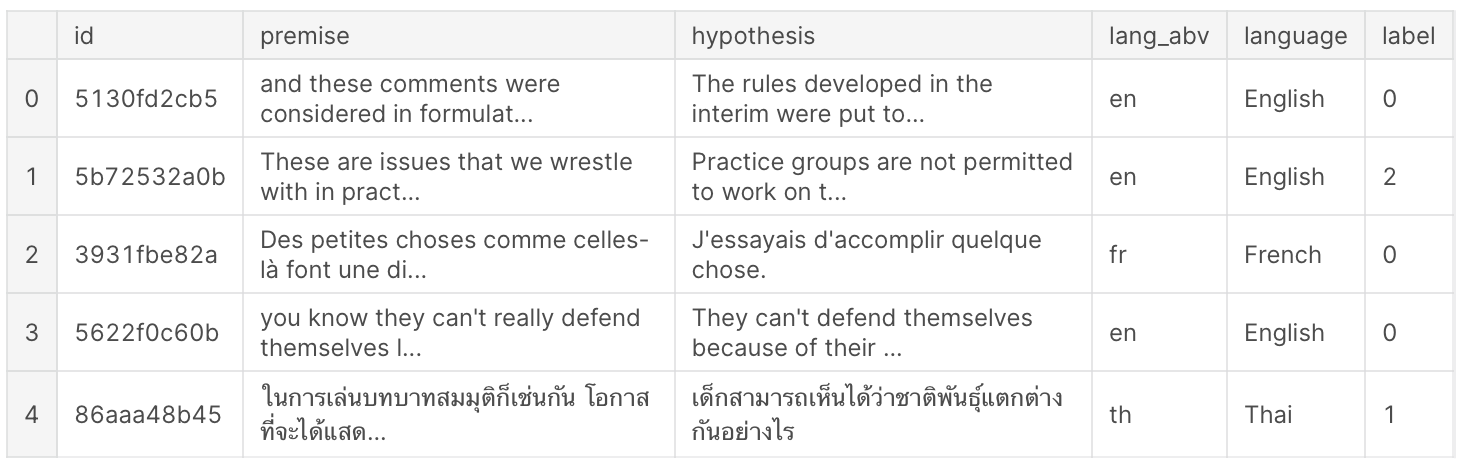
\includegraphics[width=\columnwidth]{figures/header.png}
	\caption{Header of the training set}
    \label{header}
\end{figure}

As shown in figure \ref{exploration}, the majority of sentences are in english (56.7\%). Moreover, the labels seem to be evenly spread between our three classes.

\begin{figure}[ht]
	\centering
	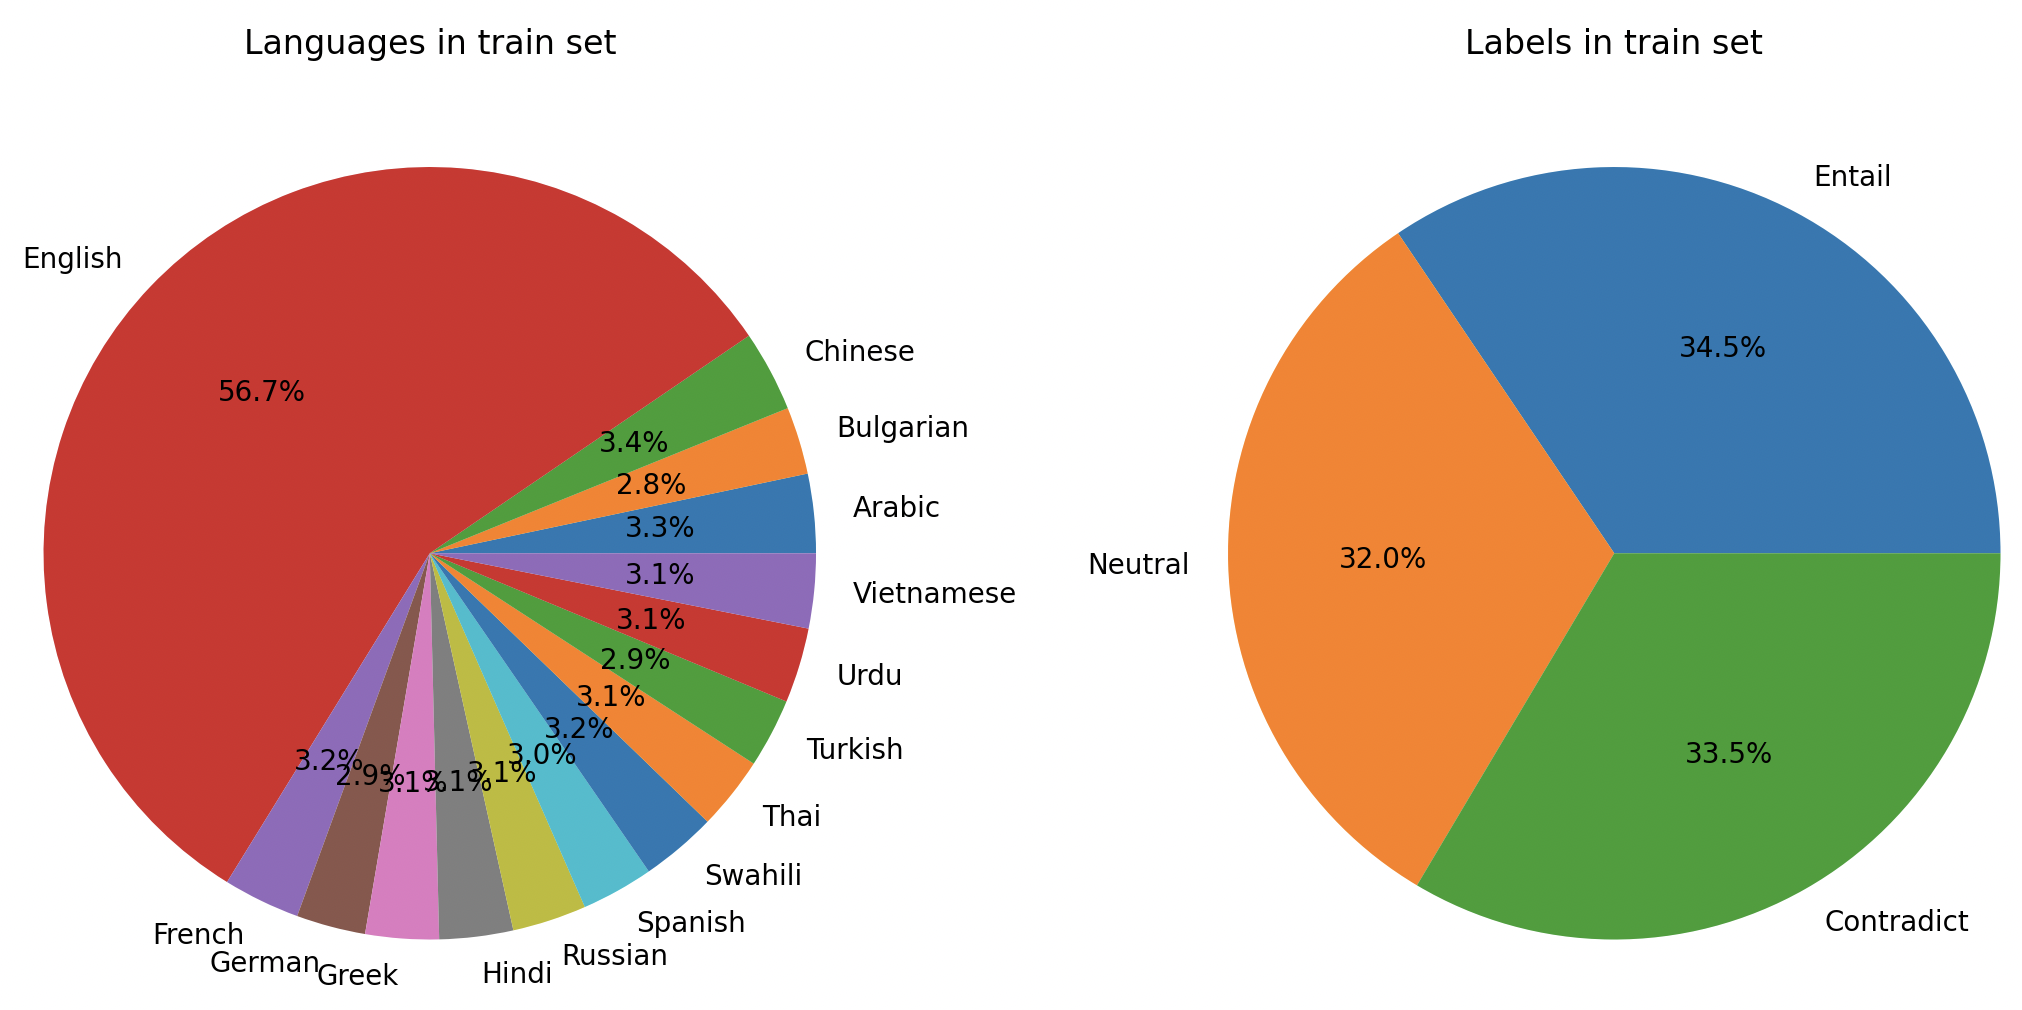
\includegraphics[width=\columnwidth]{figures/exploration.png}
	\caption{Exploration of our dataset.}
    \label{exploration}
\end{figure}

\subsection{Overview of the method}

As a reminder, our task consists in classifying pairs of sentence between three classes: entailment, neutral, and contradiction. Our objective for this task is to maximize the weighted accuracy of our classification. The general principle of our approach is the following:

\begin{itemize}
    \item Compute several features for each pair, that are relevant for our task:
    \begin{itemize}
        \item Predictions computed with a pretrained multi-lingual BERT classifier \cite{multilingualBert} fine-tuned on our datasets. These features are simply the probability for each pair of being in each class, as returned by the classifier.
        \item Hand-crafted features for our task (cf. section \ref{sec:otherFeatures} for the details). Those features are computed with embeddings of the sentences obtained with pretrained LLMs. To add variety in our pipeline, we used several different LLMs for this, which led to multiple features.
    \end{itemize}
    \item Leverage all those features to compute a final classification. We decided to use a well known gradient boosting library for this step: XGBoost \cite{xgboost}.
\end{itemize}

\begin{figure}[ht]
	\centering
	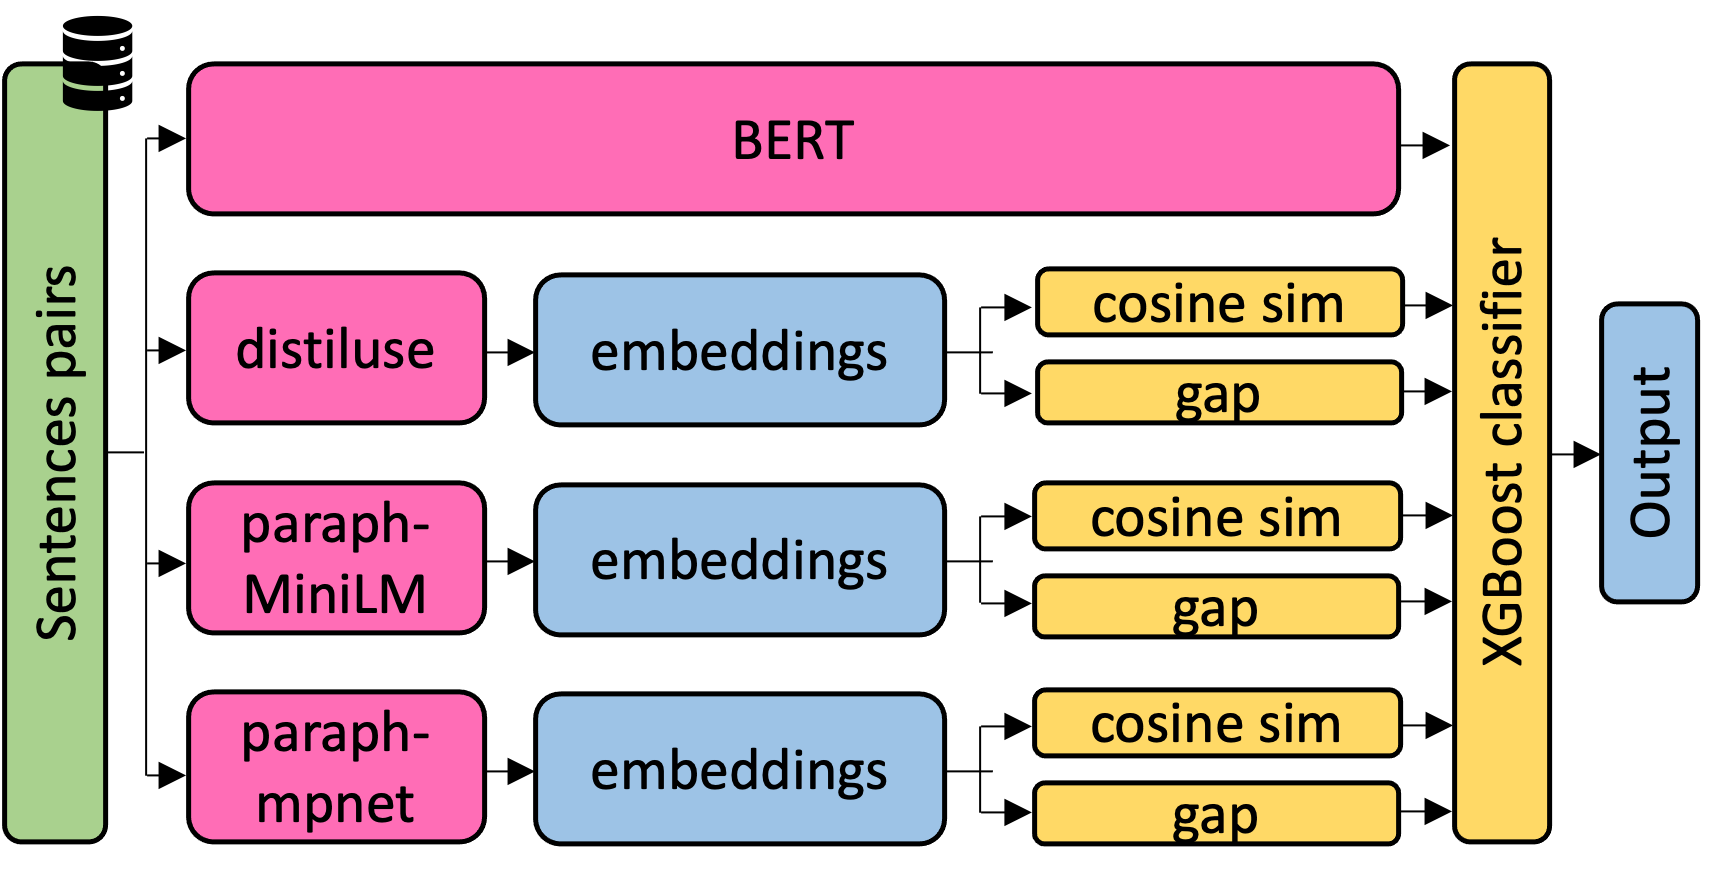
\includegraphics[width=\columnwidth]{figures/pipeline.png}
	\caption{General overview of our pipeline.}
    \label{pipeline}
\end{figure}

\subsection{First part: a multilingual BERT classifier as baseline} \label{sec:mBert}

As said before, the first part of our pipeline is a pretrained multilingual BERT classifier fine-tuned on our dataset. This part is supposed to give us a solid basis for our final classification, that will be improved with other features (cf. section \ref{sec:otherFeatures}). In this section, we will briefly recall BERT's architecture and training, and then describe how we fine-tuned it on our datasets.

\subsubsection{Brief recall: BERT's architecture and training}

BERT \cite{multilingualBert} is a transformer-based attention layer which original version was published in 2018. Contrary to directional models, which were widely used before and which read the text input sequentially (left-right or right-left), the attention layers of BERT read the entire sequence of words at once.

More precisely, if at layer $n$ each word is represented as a vector, and the sentence is represented by their aggregation in the matrix $x_n$, then the encoding at layer $n+1$ is computed as follows. This transition is called "self-attention" because the matrix $Q^TK$ represents a similarity matrix between two sets of vectors that are both computed from $x_n$: the queries $Q$ and the keys $K$.

$$
x_{n+1} = \text{softmax}\left( \frac{Q^TK}{\sqrt{d}}\right)\cdot V
$$

$$
Q = \sigma(W^Q\cdot x_n)
$$
$$
K = \sigma(W^K\cdot x_n)
$$
$$
V = \sigma(W^V\cdot x_n)
$$

Many layers like this, as well as other type of layers, are aggregated to form the architecture of BERT. Then, this architecture is trained on several unsupervised tasks:

\begin{itemize}
    \item Masking: 15\% of the words are masked and replaced by [MASK], and the network has to predict what are the masked words.
    \item Sentence prediction: The network is trained to predict the next sentence, given any input sentence from a larger corpus.
\end{itemize}

\subsubsection{Fine-tuning the model on our dataset}

For our classification task, we decided to use the transformers library \cite{transformersLib} for its simplicity. The hyperparameters we used for our training were:

\begin{itemize}
    \item Batch size: 16
    \item Metric: \texttt{eval-accuracy}
    \item Sentence max length: 512
    \item Warmup steps: 100
\end{itemize}

\subsection{Second part: features augmentation} \label{sec:otherFeatures}

\begin{figure}[ht]
	\centering
	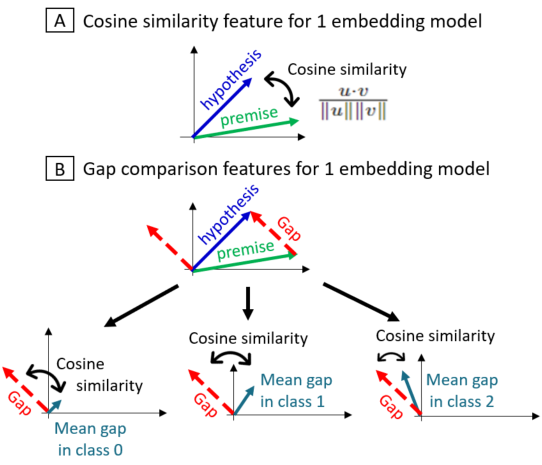
\includegraphics[width=\columnwidth]{figures/features_creation.png}
	\caption{Diagram of additional features creation process, for one embedding model. Note that 3 different embeddings where used, leading to different vector encodings and therefore to a set of $3 \times 1 + 3 \times 3 = 12$ additional features in total. A : Cosine similarity between the vector representation of the hypothesis and the premise for each pair. B : Cosine similarity between the gap (difference between the vector representation of the hypothesis and the premise) and the mean gap of each class.}
    \label{features_creation}
\end{figure}

We choose to use a special case of stacking to improve the performances of the model.

In typical stacking, a model is trained to combine the predictions of several other algorithms. In our case, we used the predictions of BERT, combined with 12 additional features that we will describe below ; finally,  we aggregated them with XGBoost. The schematics describing the creation process of those hand-crafted features is described in figure \ref{features_creation}, and explained in more details in the next paragraphs.

\subsubsection{Cosine similarity with 3 new embeddings} 

In the logic of ensemble methods, we decided to introduce embeddings computed with different models. 

We chose to use fully pre-trained models, available in the Sentence-Transformers library, in order not to increase the computation time.

We used the 3 following models: 

\begin{itemize}
    \item distiluse-base-multilingual-cased-v2
    \item paraphrase-multilingual-MiniLM-L12-v2
    \item paraphrase-multilingual-mpnet-base-v2
\end{itemize}


These three models were chosen because they are the best multilingual models trained on the languages we deal with, when evaluated on finding semantically similar sentences by \cite{reimers2020}. 

For each of the 3 embedding : 

\begin{itemize}
    \item  We computed the embeddings of each of the sentences in our dataset.
    \item We computed the cosine similarity between the embeddings of the premise and its corresponding hypothesis. Note that the cosine similarity between two vectors $u$ and $v$ is : $\frac{u \cdot v}{\|u\| \|v\|}$ 
\end{itemize}

This makes 3 new features (one cosine similarity measure for each embedding).

\subsubsection{Gap comparison} 

For each of the 3 different embeddings, we also computed the mean of the difference between the premise and the hypothesis (denoted as "gap") among each class of the train set (entailment, neutral and contradiction).

Then, for each pair of the dataset, we computed the cosine similarity between its gap and each of the mean gaps of each class. 

The idea is that among one class, the distance between the premise and the hypothesis could be generally similar (high for the contradiction class, and low for the entailment class). In high dimension, cosine similarity is generally the best notion of distance at hand. Intuitively, the distance between the premise and the hypothesis should be close from 0 in the case of entailment, and greater in the case of contradiction.

This makes $3 \times 3 = 9$ new features (one cosine similarity feature for each class and for each embedding).

\subsubsection{Aggregation using XGBoost}

Finally, we feeded XGBoost with 15 features : 

\begin{itemize}
    \item mBERT prediction for each class
    \item Our 12 new specialized features
\end{itemize}

The output is the predicted class for each pair of the dataset.

We optimized the hyperparameters of XGBoost using a grid search among 750 different parameter combinations.

\subsection{Computation resources}

For the training, we used one NVIDIA GeForce RTX 3090 24 Go. For the fine-tuning of BERT on our classification task, it took about 90 minutes and required at least 6 Go of graphic memory. For the generation of the other features based on the embeddings, the computation was really fast with GPU (about 2 minutes). Running the training on CPU is not reasonable due to the high computation time: even for the computation of the additional features based on the embeddings, this would have taken more than one hour instead of 2 minutes.

On the other hand, the final prediction with XGBoost is fast and takes few seconds on CPU, even when doing the optimal hyperparameters search.

\section{Results}


We first evaluated only the pre-trained multilingual BERT classifier. 

We fine-tuned it by training it on our train dataset. We then evaluated its performance on the validation set provided by the Kaggle challenge. We obtained 0.60 accuracy score.

We then evaluated the whole model, using the XGBoost predictions that aggregated the BERT predictions and the additional features. On the same validation set, we obtained 0.63 accuracy score.

Our diagnosis was therefore mitigated. The baseline performance of BERT was surprisingly low, as well as the final accuracy using XGBoost. However, \textbf{we obtained a $+3\%$ increase in performance using our self-engineered stacking procedure, thus validating the primary goal of our project}. Moreover, this increase in performance was achieved in a time-effective manner: only 2.3 minutes were needed to compute the new features, train the XGBoost classifier and compute the predictions ; whereas fine-tuning BERT for the baseline prediction takes 90 minutes.

We still wanted to investigate the glaring lack of performance of our baseline method, which in turns affects the performance of the final model. 

Since we validated our model on the submission set provided by Kaggle, we had no visibility on the composition of this validation set (indeed, in a Kaggle competition, the true labels of the submission set are not published). For example, we could not check whether this dataset was class-balanced or not. In the case it was class-imbalanced, we could have a drop of performance due to this fact.

We therefore amputated the provided train set to create our own validation set, ensuring that this new validation set is class-balanced. We retrained our model on this new obtained smaller train set, and evaluated it on our class-balance validation set. But we obtained the same accuracy results (to two decimal places), thus showing that our lack of performance does not come from an imbalanced validation set.

We then wondered in what extent this lack of performance comes from our multilingual setting. Our pretrained multilingual model may not perform as well as the pretrained english ones. We therefore filtered our train dataset, keeping only english sentences. We isolated a class-balanced validation set.

We used BERT based model pretrained on English language. We fine-tuned in on our training set, and we obtained 0.64 accuracy score on our validation set.

For our whole procedure, we added different embeddings to compute our special features. We kept our 3 multilingual embeddings, and we added the 4 following embeddings : 

\begin{itemize}
    \item msmarco-distilbert-cos-v5
    \item multi-qa-mpnet-base-cos-v1
    \item all-mpnet-base-v2
    \item all-distilroberta-v1
\end{itemize}

thus resulting in 7 cosine similarity features, and $7 \times 3 = 21$ gap comparison features.

When evaluating the whole procedure on our english validation set, we obtained 0.68 accuracy score.

This experiment shows that the multi-lingual setting is a more difficult task than the english one, due to the fact that current multi-lingual pretrained model do not perform as well as their english counterparts.

\section{Discussion}

In this work, we proposed a new procedure for multilingual textual entailment detection. Based on previous related work, we exploited the addition of specialised features, namely cosine similarity between premise and hypothesis using three different encodings, and comparison of the "gap" value to the mean of the gap in each class. We aggregated these additional features with the predictions of our baseline, a fine-tuned BERT classifier, using an XGBoost classifier. Using this stacking procedure, we obtained a $3\%$ increase in accuracy as compared to the baseline. This improvement is achieved in a computational effective way; only 2.3 minutes are needed to compute the additonnal features, train the XGBoost and calculate the predictions ; as compared to 90 minutes of training for the fine-tuning of BERT. These results show that our hand-crafted features are an efficient way to improve already existing textual entailment detection algorithms.

However, our absolute score remains quite low ; our baseline achieved 0.60 accuracy score, and the whole procedure achieved 0.63 accuracy score. We consequently run our pipeline with models pre-trained only on English language (filtering our datasets to keep english sentences only), and we achieved 0.64 accuracy score for the baseline, and 0.68 for the whole procedure.

This suggests the following next steps to improve those results. First, one could try another existing pre-trained algorithm for the baseline. This could include one of the models that we used to compute the additional embeddings. Another aspect to investigate would be to fine-tune the models used to compute the additionnal embeddings, by training them on our training set. This would greatly increase the computation time, but it would be interesting to understand in what extent the prediction would be more accurate.


\printbibliography


\end{document}
